%%%%%%%%%%%%%%%%%%%%%%%%%%%%%%%%%%%%%%%%%%%%%%%%%%%%%%%%%%%%%%%%%%%%%%%%%%%%%
%% Original default rstudio/pandoc latex file
%% upated by @jhollist 09/15/2014
%% inspired by @cboetting https://github.com/cboettig/template and
%% @rmflight blog posts:
%% http://rmflight.github.io/posts/2014/07/analyses_as_packages.html 
%% http://rmflight.github.io/posts/2014/07/vignetteAnalysis.html).  
%%%%%%%%%%%%%%%%%%%%%%%%%%%%%%%%%%%%%%%%%%%%%%%%%%%%%%%%%%%%%%%%%%%%%%%%%%%%%

\documentclass[11pt,a4paper]{article}
\usepackage[T1]{fontenc}
\usepackage{lmodern}
\usepackage{amssymb,amsmath}
\usepackage{ifxetex,ifluatex}
\usepackage{fixltx2e} % provides \textsubscript
% use upquote if available, for straight quotes in verbatim environments
\IfFileExists{upquote.sty}{\usepackage{upquote}}{}
\ifnum 0\ifxetex 1\fi\ifluatex 1\fi=0 % if pdftex
  \usepackage[utf8]{inputenc}
\else % if luatex or xelatex
  \ifxetex
    \usepackage{mathspec}
    \usepackage{xltxtra,xunicode}
  \else
    \usepackage{fontspec}
  \fi
  \defaultfontfeatures{Mapping=tex-text,Scale=MatchLowercase}
  \newcommand{\euro}{€}
\fi
% use microtype if available
\IfFileExists{microtype.sty}{\usepackage{microtype}}{}
\usepackage[margin=1in]{geometry}
\usepackage{longtable,booktabs}
\usepackage{graphicx}
% Redefine \includegraphics so that, unless explicit options are
% given, the image width will not exceed the width of the page.
% Images get their normal width if they fit onto the page, but
% are scaled down if they would overflow the margins.
\makeatletter
\def\ScaleIfNeeded{%
  \ifdim\Gin@nat@width>\linewidth
    \linewidth
  \else
    \Gin@nat@width
  \fi
}
\makeatother
\let\Oldincludegraphics\includegraphics
{%
 \catcode`\@=11\relax%
 \gdef\includegraphics{\@ifnextchar[{\Oldincludegraphics}{\Oldincludegraphics[width=\ScaleIfNeeded]}}%
}%
\ifxetex
  \usepackage[setpagesize=false, % page size defined by xetex
              unicode=false, % unicode breaks when used with xetex
              xetex]{hyperref}
\else
  \usepackage[unicode=true]{hyperref}
\fi
\hypersetup{breaklinks=true,
            bookmarks=true,
            pdfauthor={},
            pdftitle={working title Compatibility system and stigma size are the main predictors of heterospecific pollen effect},
            colorlinks=true,
            citecolor=blue,
            urlcolor=blue,
            linkcolor=magenta,
            pdfborder={0 0 0}}
\urlstyle{same}  % don't use monospace font for urls
\setlength{\parindent}{0pt}
\setlength{\parskip}{6pt plus 2pt minus 1pt}
\setlength{\emergencystretch}{3em}  % prevent overfull lines
\setcounter{secnumdepth}{0}

%%%%%%%%%%%%%%%%%%%%%%%%%%%%%%%%%%%%%%%%%%%%%%%%%%%%%%%%
%Changes borrowed from @cboettig, added by @jhollist 
% A modified page layout 
\textwidth 6.75in
\oddsidemargin -0.15in
\evensidemargin -0.15in
\textheight 9in
\topmargin -0.5in
\usepackage{lineno} % add 
  \linenumbers % turns line numbering on 
%%%%%%%%%%%%%%%%%%%%%%%%%%%%%%%%%%%%%%%%%%%%%%%%%%%%%%%%

%%%%%%%%%%%%%%%%%%%%%%%%%%%%%%%%%%%%%%%%%%%%%%%%%%%%%%%%
%%Packages and layout changes by @jhollist 09/15/2014
\usepackage{ragged2e}
\usepackage[font=normalsize]{caption}
  \usepackage[doublespacing]{setspace}
\usepackage{parskip}
\usepackage{fancyhdr}
\pagestyle{fancy}
\fancyhf{}
\renewcommand{\headrulewidth}{0pt}
  \rfoot{\today}
\lfoot{\thepage}
%%Changed default abstract width and added lines
\renewenvironment{abstract}{
  \hfill\begin{minipage}{1\textwidth}
  \rule{\textwidth}{1pt}\vspace{5pt}
  \normalsize
  \begin{justify}
  \bfseries\abstractname\vspace{5pt}
  \end{justify}}
  {\par\noindent\rule{\textwidth}{1pt}\end{minipage}
}
%%%%%%%%%%%%%%%%%%%%%%%%%%%%%%%%%%%%%%%%%%%%%%%%%%%%%%%%

\title{working title Compatibility system and stigma size are the main
predictors of heterospecific pollen effect}
\author{
Jose B. Lanuza, Ignasi Bartomeus, Tia-Lynn Ashman, Romina Rader
}
\date{}
% Allowing for landscape pages
\usepackage{lscape}
\newcommand{\blandscape}{\begin{landscape}}
\newcommand{\elandscape}{\end{landscape}}

% Left justification of the text: see https://www.sharelatex.com/learn/Text_alignment
% \usepackage[document]{ragged2e} % already in the latex template
\newcommand{\bleft}{\begin{flushleft}}
\newcommand{\eleft}{\end{flushleft}}

%%Fix tightlist error: https://stackoverflow.com/questions/40438037/tightlist-error-using-pandoc-with-markdown
%%Added 2018-03-26 
\providecommand{\tightlist}{%
  \setlength{\itemsep}{0pt}\setlength{\parskip}{0pt}}
%%%  
  

\begin{document}
%%Edited by @jhollist 09/15/2014
%%Adds title from YAML
\begin{singlespace}
\begin{center}
\huge working title Compatibility system and stigma size are the main
predictors of heterospecific pollen effect
\end{center}
%%Adds Author, correspond email asterisk, and affilnum from YAML
\begin{center}
\large
Jose B. Lanuza, Ignasi Bartomeus, Tia-Lynn Ashman, Romina Rader \textsuperscript{*} \textsuperscript{1,2,3} 
\end{center}
%%Adds affiliations from YAML
\begin{justify}
\footnotesize \emph{ 
\\*
\textsuperscript{1}US Environmental Protection Agency, Office of Research and Development,
National Health and Environmental Effects Research Laboratory, Atlantic
Ecology Division, 27 Tarzwell Drive Narragansett, RI, 02882, USA\\*
\\*
\textsuperscript{2}Big Name University, Department of R, City, BN, 01020, USA\\*
\\*
\textsuperscript{3}Estacion Biologica de Donana (EBD-CSIC), E-41092 Sevilla, Spain\\*
}
%%Adds corresponding author email(s) from YAML
\newcounter{num}
\setcounter{num}{1}
\\[0.1cm]
\footnotesize \emph{ 
\ifnum\value{num}=1%
\textsuperscript{*} corresponding author:
\fi
\href{mailto:barragansljose@gmail.com}{\nolinkurl{barragansljose@gmail.com}}
\stepcounter{num}
}
\end{justify}
%%Adds date from YAML
\normalsize

\end{singlespace}


\singlespace

\vspace{2mm}\hrule

Pollinator sharing can have negative consequences for plant fitness with
the arrival of foreign pollen. However, the costs of heterospecific
pollen are not yet well understood. We conducted a glasshouse experiment
to understand how phylogenetic relatedness and plant traits mediate the
impacts of heterospecific pollen transfer. We conducted 1800 crosses by
experimentally transferring pollen (50\% and 100\% ratio) with
reciprocal crosses between 10 species belonging to three different
families: Brassicaceae, Solanaceae and Convolvulaceae. Seed set was used
as proxy of plant fitness. We found that for 65\% of the treatments with
50\% mix reduced seed set. Moreover, the reduction in seed set was
dependent on the degree of relatedness and reproductive traits of the
pollen recipient and not the pollen donor. Our results show that certain
traits, particularly compatibility system, are critical in understanding
the costs of heterospecific pollen. \vspace{3mm}\hrule

\emph{Keywords}: heterospecific pollen, plant reproduction, fitness,
interspecific competition, phylogenetic distance.

\doublespace

\bleft

\section{INTRODUCTION}\label{introduction}

In most ecosystems, plant species normally coexist and share their
floral visitors with other species Waser et al. (1996). From the plants'
perspective, pollinator sharing can be positive for some plants
Carvalheiro et al. (2014) or negative for others Pauw (2013), depending
on the facilitation gradient. An increasing number of visits often
correlates with higher chances of fertilization Engel and Irwin (2003).
However this is not always the case, among these possible flower
visitors there are also nectar robbers and pollen thieves Inouye (1980);
Magrach et al. (2017). Receiving both sufficient quantity and quality
deposited on the stigma is thus highly relevant to the pollination
success of the plant Aizen and Harder (2007).

By visiting many plant species, many pollinators are responsible for
conspecific pollen loss and the transport of foreign pollen, both of
which can have important detrimental effects on species fitness Morales
and Traveset (2008); Ashman and Arceo-Gómez (2013); Arceo-Gómez and
Ashman (2016). Foreign pollen arrival can play an important role in
plant species fitness but outcomes are variable and appear to be context
dependent as there is not always a decrease in fitness Morales and
Traveset (2008). Some of this variation is likely due to the enormous
variability of foreign pollen transferred across systems ranging from 0
to 75 percent. However, most studies report ranges of heterospecific
pollen between 0 and 20 percent of the total pollen load Bartomeus et
al. (2008) Montgomery and Rathcke (2012); Ashman and Arceo-Gómez (2013);
Fang and Huang (2013), yet even these relatively low amounts of
heterospecific pollen transferred can decrease fitness greatly Thomson
et al. (1982). While we now have some understanding of the impacts of
heterospecific pollen quantity, we have less understanding of other
factors that could be driving the variation in impacts upon fitness.
Ashman and Arceo-Gómez (2013) postulated the first predictive framework
that identifies a need to understand how plant traits might mediate
heterospecific pollen effect, whereby mating system and pollen size were
predicted to potentially mediate the impact of foreign pollen transfer
on plant fitness. This concept is supported by specific case studies,
such as Tong and Huang (2016) that demonstrate an asymmetrical effect in
6 species of \emph{Pedicularis} whereby the pollen of long styled
species was able to grow the full length of the style on short styled
species but not vice versa. While this suggests that the impacts of
heterospecific pollen may differ among pollen donor and recipient, few
studies have been conducted to ascertain whether this pattern is in fact
a general trend or to identify the extent to which other plant traits
are critical to heterospecific pollen impacts.

Plant traits are crucial to understand heterospecific pollen effect but
the multifactorial nature of the traits that are involve in the
pollen-pistil interaction make difficult to unravel what are the main
traits in driving the effect. These traits can be seen from a male
perspective of both donor and recipient where pollen size, pollen
aperture number and pollen allelopathy are key components to understand
the outcome of foreign pollen arrival Murphy and Aarssen (1995); Ashman
and Arceo-Gómez (2013). In Ashman and Arceo-Gómez (2013) small pollen is
predicted to cause a greater fitness decrease, although this can be true
there are also other possibilities to consider which can obscure a
predictive framework like big pollen can clogg small stigmas with fewer
pollen grains, bigger stigmas are less likely to be clogged by small
pollen grains and bigger pollen can outcompete smaller pollen grains due
to faster pollen tube growth rate Williams and Rouse (1990). Moreover,
to understand the different mechanical or chemical effects of pollen
also the female traits of the pollen recipient have to be considered,
from the literature these main traits are: stigma size, style length,
number of ovules, incompatibility system and also a structural trait
such as flower morphology Montgomery and Rathcke (2012); Ashman and
Arceo-Gómez (2013); Tong and Huang (2016). For example, greater
stigmatic area is positively correlated with greater heterospecific
pollen deposition Montgomery and Rathcke (2012) and therefore possibly
with an increase in negative effect. For species that are
self-incompatible the barriers towards heterospecific pollen are
stronger than self-compatible species Ashman and Arceo-Gómez (2013).
Nonetheless, an effect of foreign pollen is a bit obscured by the
variability within species, however species that are strong selfers or
strong outcrossers have less variablity in mating systems and
predictions of effect could be more realistic (see figure 1 from
Whitehead et al. (2018)). Although past research has progress in the
understanding of what traits can mediate the effect as we have shown
here, there are multiple traits involved and multiple possible scenarios
still to be explored empirically for a full understanding of the
importance of heterospecific pollen effect in nature.

For the understanding at what level or intensity the interference of
pollen can occur is important to consider the relatedness of the
interacting species. Closely related species are more likely to have
similar traits Letten and Cornwell (2015). The similarity in traits
between closely related species can lead to higher chances of ovule
usurpation/abortion Arceo-Gómez and Ashman (2011) and therefore studies
predict and show a greater negative effect of closely related species
Ashman and Arceo-Gómez (2013); Arceo-Gómez and Ashman (2016). Few
studies however, have focused on the impacts of heterospecific pollen on
fitness of distantly related species Galen and Gregory (1989); Neiland
and Wilcock (1999). Despite the fact that far related species are also
able to decrease species fitness (REFS). Yet, most insects and most
stigmas have been found to carry multiple species of foreign pollen with
little attention to degree of relatedness (Arceo-Gómez and Ashman
(2016); Fang and Huang (2013). Understanding the role of foreign pollen
from distantly related species thus deserves greater attention. The
relatedness of foreign pollen gives a first snapshoot of where the
pollen competition can occur and therefore could be a proxy of effect.
With that said, Arceo-Gómez and Ashman (2016) is the only work which has
proven a greater effect of close related species through a meta-analysis
but with low sample sizes and lack of significance. Therefore, there is
a need to study the effect of heterospecific pollen of far and close
related species at community level beyond single pairwise interactions.

Heterospecific pollen studies in nature have the complexity added of
great environmental variability which can lead to confounding
interpretations. Moreover, the great diversity of floral structures and
small sizes of some of them such as Asteraceae species make tedious or
almost impossible the studies of heterospecific pollen on the field. For
this reason, we investigated how floral reproductive traits and
relatedness mediate the impact of heterospecific pollen by creating an
artificial co-flowering community in a glasshouse with 10 species
belonging to three different families with different traits. Our study
tries to answer the following questions: (i) Do heterospecific pollen
reduce seed set? To what extent do (ii) floral reproductive traits and
(iii) relatedness, mediate the impacts of heterospecific pollen on seed
set.

\section{METHODS}\label{methods}

The study was conducted in a glasshouse at University of New England
(Armidale, Australia) from November 2017 to March 2018. Rooms were
temperature controlled depending on the requirements of the species with
day and night temperature differences. The experimental design had
species from three different families: Solanaceae, Brassicaceae and
Convolvulaceae (\textbf{Table 1}). The species of the study had
different reproductive traits and different degree of relatedness where
the reciprocal crosses between species allowed us to have multiple
different scenarios of both traits and relatedness. Moreover, the
species selected had fast life cycle and low structural flower
complexity in order to perform the pollination treatments and grow the
different species from seeds. For the purpose of the experiment all the
species where considered as pollen recipient and as pollen donor (see
interaction matrix, fig 2). Species were watered once or twice per day
and fertilized weekly (NPK 23: 3.95: 14).

\textbf{Table 1}

\begin{longtable}[]{@{}lll@{}}
\toprule
Family & Genus & Species\tabularnewline
\midrule
\endhead
Brassicaceae & Brassica & Brassica rapa\tabularnewline
Brassicaceae & Brassica & Brassica oleracea\tabularnewline
Brassicaceae & Eruca & Eruca versicaria\tabularnewline
Brassicaceae & Sinapis & Sinapis alba\tabularnewline
Convolvulaceae & Ipomoea & Ipomoea aquatica\tabularnewline
Convolvulaceae & Ipomoea & Ipomoea purpurea\tabularnewline
Solanaceae & Capsicum & Capsicum annuum\tabularnewline
Solanaceae & Petunia & Petunia integrifolia\tabularnewline
Solanaceae & Solanum & Solanum lycopersicum\tabularnewline
Solanaceae & Solanum & Solanum melongena\tabularnewline
\bottomrule
\end{longtable}

\textbf{Hand-pollination}

Foreign pollen effect was studied through two different treatments, one
with 50\% conspecific pollen and 50\% heterospecific pollen and a second
one with 100\% foreign pollen (N=10) in order to see if foreign pollen
can trigger fruit production by itself or even seeds through ovule
usurpation. Therefore, 180 different combinations were performed with
N=10 per combination. Seed set was the proxy of effect for all our
treatments. Moreover, hand cross pollination (between individuals of the
same species), hand self pollination, apomixis (bagged emasculated
flowers) and natural selfing were tested for each species (N=10). For
the treatments with foreign pollen and hand cross pollination, flowers
were emasculated the day prior anthesis and hand pollinated next day
with a toothpick. Hand-pollination was conducted with 3-4 gentle touches
on the stigma surface. For each species 20 anthers were collected and
their pollen counted with a hemocytometer, each anther was counted 4
times and then an average of these counts was performed. Once, the
average number of pollen grains per anther was known, the proportion of
anthers per mix was calculated in order to achieve a 50-50\% mix. In
order to confirm that the treatments applied were the desire
proportions, for each focal species the total stigmatic load of pollen
was counted from one donor of each family (N=3).

\textbf{Traits and evolutive distance}

The traits measured for each species were pollen per anther, number of
ovules and stigma, style, ovary width and length. For the stigma, the
stigmatic area was also measured and moreover the stigmas were divided
in wet/dry type. All the morphometrical measurements were performed with
a stereophotomicroscope. Pollen was counted for 20 anthers of each
species with 4 replicates per sample with an hemocytometer. Previously,
anthers were squashed on a known solution with the pippete tip and
homogeneize with a vortex for 30 seconds. Ovule number was counted with
the help of a stereomicroscope and a small grid over a petri dish from
15 randomly selected flowers. Fruits per number of flowers treated were
counted for Solanaceae species and for the rest, the number of seeds
produced per average number of ovules of each species. Levels of self
incompatibility were estimated by dividing the fruit set of hand self
pollination by hand cross pollination Lloyd and Schoen (1992).

\textbf{Analysis}

To evaluate heterospecific pollen effect on seed production we performed
linear mixed models. The distinct heterospecific pollination treatments
were compared through relevelling each variable with the cross
pollination treatment which was our control for optimum seed production
for all the species. The different replicates of each treatment were
considered as random effects. Seed production was scaled for all the
species with mean 0 and standard deviation of 1 prior to the analysis.
All the analysis were conducted with the statistical language \texttt{R}
(R Core Team 2018).

In order to test the relative effect of traits on seed production with
foreign pollen we performed Mantel test between the assymetrical matrix
of heterospecific pollen effect (10 by 10 matrix) with the different
distance matrices of traits (Euclidean distances). Heterospecific pollen
effect was obtained through the subtraction of seed production by hand
cross pollination minus seed production of the different heterospecific
pollen treatments. To find a model with the best explanatory traits we
used the function \textbf{bioenv} from R. We also conducted Mantel test
between the matrix of heterospecific pollen effect and the distance
matrix from all the traits. Moreover, we explored also the correlation
between traits and heterospecific pollen effect through generalized
mixed models where the response variable was heterospecific pollen
effect and the explanatory variable the different traits.

We conducted mantel test to check for correlations between
heterospecific pollen effect and phylogenetic distance. Due to
improvents in statistical power we used the square root of the
phylogenetic distance (Letten \& Cornwell 2014). Two different
phylogenetic distances were used from two kinds of markers: 1) Internal
transcribed spacer (ITS) and 2) ribulose-bisphosphate carboxylase
(RBCL). The sequences were obtained from GenBank
(\url{https://www.ncbi.nlm.nih.gov/genbank/}, accessed 20 Oct. 2018).
The sequences were aligned with clustal omega and the pairwise evolutive
distances calculated with MEGA7.

\href{Jose}{Phylogenetic signal of traits?}

\section{RESULTS}\label{results}

Results of hand cross-pollination, self hand-pollination, natural
selfing and apomixis are presented in \textbf{Figure 1} (see appendix 1
for table with values). Heterospecific pollen reduced seet set
significatively with the 50-50\% heterospecific pollen treatments for
65\% of the pairwise interactions p\textless{}0.05.

Across families we found a very similar effect but when species where
look at species level they respond differently even within the same
family \href{}{rephrase and maybe test statistically?}, for instance for
two species of the Brassicaceae family \emph{Brassica oleracea} and
\emph{Eruca versicaria} we found very contrasting effects of foreign
pollen where for the first one, all donors reduce seed set
significatively and for the second, just two species did out of nine.
The 100\% foreign pollen treatments barely produced seeds or fruits
\href{}{and just for \emph{Sinapis alba} we did not find significant
differences between the hand cross pollination and one treatment with
pollen from a confamilial- IB Unclear}. Solanaceae species with berry
fruit type developed small fruits or even normal fruits in some cases
\href{}{under which treatment}. \emph{S. lycopersicum} seems to produced
small fruits (35\% of the treatments) independently of pollen and pollen
donor due to also apomictic treatments did, never normal size. \emph{C.
annuum} produced some fruits (9\%) of both small and normal size and
finally \emph{S. melongena} produced seedless normal fruits with just
confamilial pollen (3\%), for both species seems that fruit formation
was induced by pollen on the stigma because of lack of fruit production
with treatments that tested for apomixis.\href{}{clarify this
descriptive statistics part- Also a figure with a summary of the
treatments effect would be cool, or at least in the appendices}

\newpage

\begin{figure}
\centering
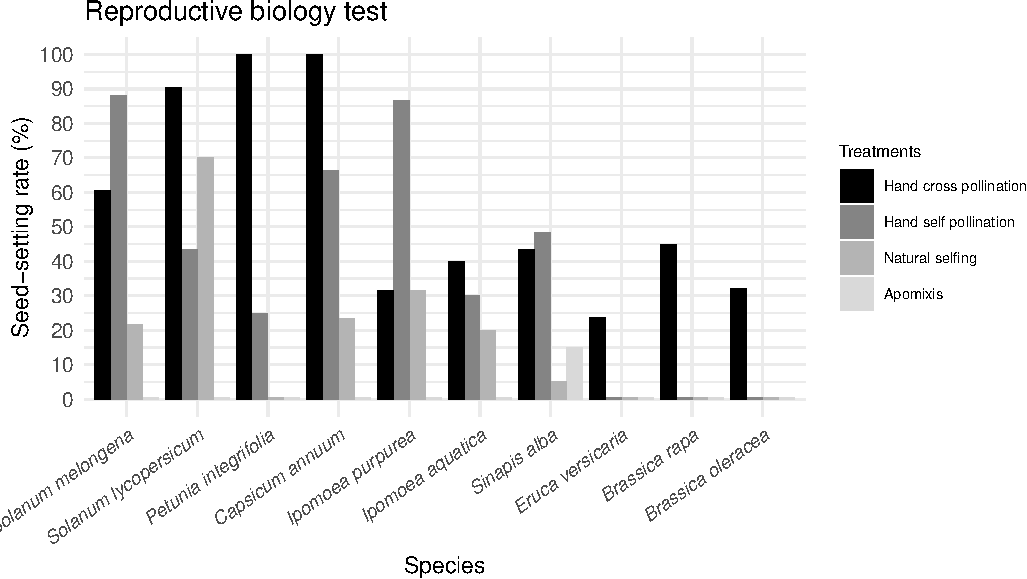
\includegraphics{output/figures/unnamed-chunk-2-1.pdf}
\caption{Barplot with the different treatments that provide information
of the reproductive biology of the ten species. The y axis is the
proportion of ovules converted to seed in percentage. The different
treatments (N=10) which are presented in the legend are, hand cross
pollination, hand self pollination, natural selfing and apomixis. More
information about these treatments can be found in Methods and
Appendices.}
\end{figure}

\newpage

Mantel test indicates that a possible?? \href{}{It exists!} correlation
exist between heterospecific pollen effect and the evolutive relative
distances, for ITS and RBCL markers we had r coefficients of 0.29 and
0.25 respectively p\textless{}0.05 \href{}{think on a figure - maybe
using NMDS}. Moreover, Mantel test indicates that also a possible??
correlation between stigma width and stigma type exist (stats??). Trait
correlations were also explored with GLMM

\href{Jose}{I have done it at the moment just for Compatibility system}
\href{Jose}{Also I have to fix from mixed linear model to GLMM, just
realize that}

\newpage

\begin{figure}
\centering
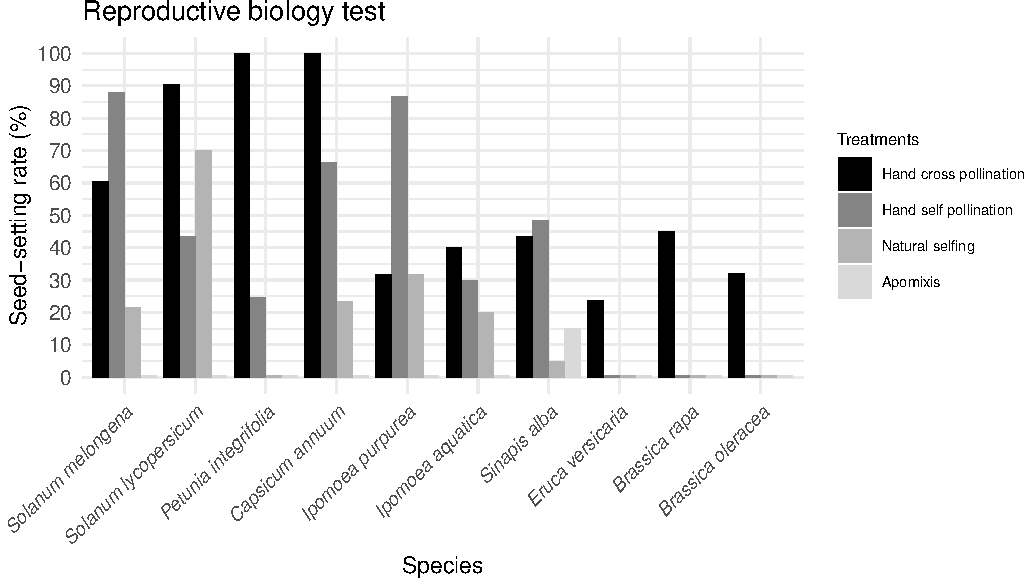
\includegraphics{output/figures/unnamed-chunk-3-1.pdf}
\caption{The effect of heterospecific pollen (scaled see set) is
represented in function of the compatibility system (self/cross*100) for
the the different species. Each coulored dot represents the interaction
of a focal species with a different pollen donor.}
\end{figure}

\href{Jose}{Compatibility index don´t multiply per 100 from Lloyd}

\newpage

\section{DISCUSSION}\label{discussion}

Discussion

Herbs vs tress, annual vs perennial\ldots{} Many flowers vs few flowered
species; structural composition on a system

What are the implications of the findings?

Ideas about pollen size in heterospecific pollen effect. (still have to
develop it more\ldots{})

Let's classify pollen size in three groups in order to understand the
interaction between pollen donor and recipient: 1) Donor pollen size
\textless{} Recipient pollen size 2) Donor pollen size = Recipient
pollen size 3) Donor pollen size \textgreater{} Recipient pollen size

Now I try to develop each part

\begin{enumerate}
\def\labelenumi{\arabic{enumi})}
\tightlist
\item
  Donor pollen size \textless{} Recipient pollen size
\end{enumerate}

Effect:

\begin{itemize}
\item
  Donor's pollen could clogg the stigma
\item
  Chemical inhibition
\end{itemize}

Traits associated with bigger pollen of the recipient:

\begin{itemize}
\item
  Recipient's pollen have faster pollen tube growth (example with my
  data)
\item
  Reduction in number of ovules (Also with my species)
\item
  Big differences in pollen size can be traduced in low relatednes
  therefore less likely of pollen germination on a far related stigma.
\end{itemize}

\begin{enumerate}
\def\labelenumi{\arabic{enumi})}
\setcounter{enumi}{1}
\tightlist
\item
  Donor pollen size = Recipient pollen size
\end{enumerate}

\begin{itemize}
\item
  Very relatedness dependant this point
\item
  Similar probabilities of taken space on the stigma
\end{itemize}

\begin{enumerate}
\def\labelenumi{\arabic{enumi})}
\setcounter{enumi}{2}
\tightlist
\item
  Donor pollen size \textgreater{} Recipient pollen size
\end{enumerate}

Effect:

-In small stigmas big pollen grains can occupy great part of the
stigmatic area.

-small pollen grains can get embeded

IB: Think also on using tree analysis to test if hp effect depends on
complex trait combinations. Tree analysis are great when two different
strategies lead to the same outcome. This would never been pick up by
GLMs. The r package is party\{\} . You can see an example applied to
birds is Sol et al 2010 Science. Ask me if you want more details or code
examples.

\section{CONCLUSIONS}\label{conclusions}

\section{ACKNOWLEDGEMENTS}\label{acknowledgements}

\section{REFERENCES}\label{references}

\hypertarget{refs}{}
\hypertarget{ref-aizen2007}{}
Aizen, M. A., and L. D. Harder. 2007. Expanding the limits of the
pollen-limitation concept: Effects of pollen quantity and quality.
Ecology 88:271--281.

\hypertarget{ref-arceo2011}{}
Arceo-Gómez, G., and T.-L. Ashman. 2011. Heterospecific pollen
deposition: Does diversity alter the consequences? New Phytologist
192:738--746.

\hypertarget{ref-arceo2016}{}
Arceo-Gómez, G., and T.-L. Ashman. 2016. Invasion status and
phylogenetic relatedness predict cost of heterospecific pollen receipt:
Implications for native biodiversity decline. Journal of Ecology
104:1003--1008.

\hypertarget{ref-ashman2013}{}
Ashman, T.-L., and G. Arceo-Gómez. 2013. Toward a predictive
understanding of the fitness costs of heterospecific pollen receipt and
its importance in co-flowering communities. American Journal of Botany
100:1061--1070.

\hypertarget{ref-bartomeus2008}{}
Bartomeus, I., J. Bosch, and M. Vilà. 2008. High invasive pollen
transfer, yet low deposition on native stigmas in a carpobrotus-invaded
community. Annals of Botany 102:417--424.

\hypertarget{ref-carvalheiro2014}{}
Carvalheiro, L. G., J. C. Biesmeijer, G. Benadi, J. Fründ, M. Stang, I.
Bartomeus, C. N. Kaiser-Bunbury, M. Baude, S. I. Gomes, V. Merckx, and
others. 2014. The potential for indirect effects between co-flowering
plants via shared pollinators depends on resource abundance,
accessibility and relatedness. Ecology letters 17:1389--1399.

\hypertarget{ref-engel2003}{}
Engel, E. C., and R. E. Irwin. 2003. Linking pollinator visitation rate
and pollen receipt. American Journal of Botany 90:1612--1618.

\hypertarget{ref-fang2013}{}
Fang, Q., and S.-Q. Huang. 2013. A directed network analysis of
heterospecific pollen transfer in a biodiverse community. Ecology
94:1176--1185.

\hypertarget{ref-galen1989}{}
Galen, C., and T. Gregory. 1989. Interspecific pollen transfer as a
mechanism of competition: Consequences of foreign pollen contamination
for seed set in the alpine wildflower, polemonium viscosum. Oecologia
81:120--123.

\hypertarget{ref-inouye1980}{}
Inouye, D. W. 1980. The terminology of floral larceny. Ecology
61:1251--1253.

\hypertarget{ref-letten2015}{}
Letten, A. D., and W. K. Cornwell. 2015. Trees, branches and (square)
roots: Why evolutionary relatedness is not linearly related to
functional distance. Methods in Ecology and Evolution 6:439--444.

\hypertarget{ref-lloyd1992}{}
Lloyd, D. G., and D. J. Schoen. 1992. Self-and cross-fertilization in
plants. i. functional dimensions. International Journal of Plant
Sciences 153:358--369.

\hypertarget{ref-magrach2017}{}
Magrach, A., J. P. González-Varo, M. Boiffier, M. Vilà, and I.
Bartomeus. 2017. Honeybee spillover reshuffles pollinator diets and
affects plant reproductive success. Nature ecology \& evolution 1:1299.

\hypertarget{ref-montgomery2012}{}
Montgomery, B. R., and B. J. Rathcke. 2012. Effects of floral
restrictiveness and stigma size on heterospecific pollen receipt in a
prairie community. Oecologia 168:449--458.

\hypertarget{ref-morales2008}{}
Morales, C. L., and A. Traveset. 2008. Interspecific pollen transfer:
Magnitude, prevalence and consequences for plant fitness. Critical
Reviews in Plant Sciences 27:221--238.

\hypertarget{ref-murphy1995}{}
Murphy, S. D., and L. W. Aarssen. 1995. Reduced seed set in elytrigia
repens caused by allelopathic pollen from phleum pratense. Canadian
Journal of Botany 73:1417--1422.

\hypertarget{ref-neiland1999}{}
Neiland, M., and C. Wilcock. 1999. The presence of heterospecific pollen
on stigmas of nectariferous and nectarless orchids and its consequences
for their reproductive success. Protoplasma 208:65--75.

\hypertarget{ref-pauw2013}{}
Pauw, A. 2013. Can pollination niches facilitate plant coexistence?
Trends in ecology \& evolution 28:30--37.

\hypertarget{ref-R_Core_Team_2018}{}
R Core Team. 2018. R: A language and environment for statistical
computing. R Foundation for Statistical Computing, Vienna, Austria.

\hypertarget{ref-thomson1982}{}
Thomson, J. D., B. J. Andrews, and R. Plowright. 1982. The effect of a
foreign pollen on ovule development in diervilla lonicera
(caprifoliaceae). New Phytologist 90:777--783.

\hypertarget{ref-tong2016}{}
Tong, Z.-Y., and S.-Q. Huang. 2016. Pre-and post-pollination interaction
between six co-flowering pedicularis species via heterospecific pollen
transfer. New Phytologist 211:1452--1461.

\hypertarget{ref-waser1996}{}
Waser, N. M., L. Chittka, M. V. Price, N. M. Williams, and J. Ollerton.
1996. Generalization in pollination systems, and why it matters. Ecology
77:1043--1060.

\hypertarget{ref-whitehead2018}{}
Whitehead, M. R., R. Lanfear, R. J. Mitchell, and J. D. Karron. 2018.
Plant mating systems often vary widely among populations. Frontiers in
Ecology and Evolution 6:38.

\hypertarget{ref-williams1990}{}
Williams, E., and J. Rouse. 1990. Relationships of pollen size, pistil
length and pollen tube growth rates in rhododendron and their influence
on hybridization. Sexual Plant Reproduction 3:7--17.

\section{APPENDIX}\label{appendix}

\begin{enumerate}
\def\labelenumi{\arabic{enumi}.}
\item
\end{enumerate}

\textbf{Table S1}. Perecentage of seeds produced per ovule for the ten
species used in the experiment. The treatments presented are hand cross
pollination, hand self pollination, natural selfing and apomixis
(emasculated flowers).

\begin{longtable}[]{@{}lrrrr@{}}
\toprule
Species & Cross & Self & Natural\_selfing & Apomixis\tabularnewline
\midrule
\endhead
Brassica oleracea & 32.06897 & 0.0000000 & 0.00000 & 0\tabularnewline
Brassica rapa & 44.97041 & 0.0000000 & 0.00000 & 0\tabularnewline
Eruca versicaria & 23.75000 & 0.4166667 & 0.00000 & 0\tabularnewline
Sinapis alba & 43.33333 & 48.3333333 & 5.00000 & 15\tabularnewline
Ipomoea aquatica & 40.00000 & 30.0000000 & 20.00000 & 0\tabularnewline
Ipomoea purpurea & 31.66667 & 86.6666667 & 31.66667 & 0\tabularnewline
Capsicum annuum & 100.00000 & 66.2240664 & 23.48548 & 0\tabularnewline
Petunia integrifolia & 100.00000 & 24.7727273 & 0.00000 &
0\tabularnewline
Solanum lycopersicum & 90.38043 & 43.4782609 & 70.00000 &
0\tabularnewline
Solanum melongena & 60.47525 & 87.9702970 & 21.56436 & 0\tabularnewline
\bottomrule
\end{longtable}

\eleft

\clearpage

\listoftables

\newpage

\newpage

\clearpage

\listoffigures

\newpage

\newpage

\blandscape

\elandscape

\clearpage

\end{document}